\section{Caso de estudio trivariado:  orientaci\'on-longitud-apertura.}
\label{s:caseStudy3D}

Para mostrar la utilidad de esta teor\'ia se gener\'o computacionalmente un sistema de fracturas (\autoref{f:fracAbs}) al cual se le dio una estructura de dependencia compleja en el que las fracturas en la direcci\'on vertical son m\'as peque\~nas que las que est\'an en direcci\'on horizontal. Adem\'as, la relaci\'on longitud-apertura es mon\'otona, aunque no lineal (\autoref{f:psdObs}). Por otro lado, la ubicaci\'on espacial fue simulada mediante un proceso puntual de Poisson con intensidad constante ya que un proceso de Poisson con intensidad variable no permiti\'o una mejor visualizaci\'on de la red de fracturas. Los par\'ametros de los modelos se muestran a continuaci\'on:

\begin{figure}[H]
\centering
\includegraphics[height=0.4\textwidth,  keepaspectratio = TRUE]{DFN-1}
\caption{Sistema de fracturas a analizar.}
\label{f:fracAbs} % 'frac'ture 'abs'traction = conceptual model
\end{figure}

\begin{itemize}
  \item $x - poisproc(I = 0.5)$
  	\item $\theta - vonmises(\mu = 90, 180; \kappa = 10, 10))$
  \item $L - lnorm(\mu = 4, 2; \sigma = 0.4, 0.6)$
    \item $b - lnorm(\mu = exp(-4); \sigma = exp(1))$
\end{itemize}

N\'otese que tanto los datos de orientaci\'on como los datos de longitud fueron simulados cada uno como una combinaci\'on de las distribuciones de probabilidad correspondientes, lo que resulta en distribuciones bimodales tanto para los \'angulos como para las longitudes. La relaci\'on de dependencia entre estas dos variables (\autoref{f:psdObs}) parece f\'acil ya que es una uni\'on de dependencia lineal y uniforme, sin embargo, en la pr\'actica es dif\'icil modelarla cuando se dan de esta manera.

Por fines de comparaci\'on con simulaciones de este mismo sistema de fracturas, a continuaci\'on, se muestran algunos estad\'igrafos del an\'alisis exploratorio de los datos. Las direcciones de las fracturas est\'an medidas en un rango de 0$^\circ$ a 180$^\circ$ sobre un sistema de coordenadas geogr\'afico. Los estad\'igrafos de la variable direccional $\Theta$ fueron calculados mediante la estad\'istica de datos orientados \citep{mardia_directional_2000,fisher_statistical_1995,jammalamadaka_topics_2001}.

\begin{table}[htpb]
\begin{center}
	\begin{tabular}{|c|c|c|} % r = right aligment, c = centered
		\hline % adds a horizontal line
		\textbf{Estad\'igrafos} & \textbf{$L$} & \textbf{$\theta$} \\
		\hline\hline
		$\mu$    & 34.6203 & 36.3756 \\
		Mediana   & 24.1315 & 36.5734 \\
		$\sigma$ & 30.3200 & 59.5328 \\
		Asimetr\'ia & 0.8456  & -0.2369 \\ \hline
	\end{tabular}
\end{center}
    \caption{Estad\'igrafos de las longitudes y las orientaciones. Los estad\'igrafos de $\theta$ fueron estimados mediante la estad\'istica de datos orientados. Comp\'arese con la \autoref{tab:trivSim}.}
    \label{tab:triv}
\end{table}

N\'otese que estos estad\'igrafos no representan adecuadamente los modelos ya que no son modelos univariados. Sin embargo, se espera que la metodolog\'ia presentada s\'i logre reproducir cada uno de los ingredientes para generar esta red de fracturas, as\'i como los estad\'igrafos.

\begin{figure}
	\centering
	\includegraphics[width=0.8\textwidth,  keepaspectratio = TRUE]{x-1}
	\caption{Matrix de diagramas de dispersi\'on con las correspondientes distributiones marginales en las entradas de la diagonal.}
\end{figure}

\begin{figure}
	\centering
	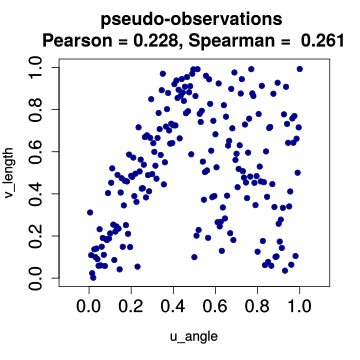
\includegraphics[height=0.4\textwidth,  keepaspectratio = TRUE]{empCopScatter-1}
	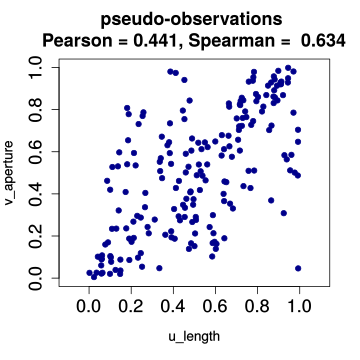
\includegraphics[height=0.4\textwidth,  keepaspectratio = TRUE]{empCopScatter-2}
	\caption{Diagramas de dispersi\'on de las pseudo-observaciones.}
	\label{f:psdObs} % Pseudo observaciones
\end{figure}

Con los datos de la \autoref{f:fracAbs} se model\'o de manera separada: a) la distribuci\'on marginal de las orientaciones, b) la distribuci\'on marginal de las longitudes, c) la distribuci\'on marginal de las aperturas, d) la c\'opula de la relaci\'on orientaci\'on-longitud, e) la c\'opula longitud-apertura.
Estos \'ultimos dos incisos se llevaron a cabo suponiendo independencia condicional.

Uno de los objetivos buscados al modelar vectores aleatorios es simular realizaciones del mismo proceso subyacente. A continuaci\'on, se muestra el resultado de una simulaci\'on.
\begin{table}[htpb]
\begin{center}
	\begin{tabular}{|c|c|c|} % r = right aligment, c = centered
		\hline % adds a horizontal line
		\textbf{Estad\'igrafos} & \textbf{$L$} & \textbf{$\theta$} \\
		\hline\hline
		$\mu$    & 38.1409 & 51.8984\\
		Mediana   & 32.6340 & 55.5260\\
		$\sigma$ & 31.0912 & 55.5536\\
		Asimetr\'ia & 0.7451  & 0.2844 \\ \hline
	\end{tabular}
\end{center}
    \caption{Estad\'igrafos de las longitudes y las orientaticiones de las simulaciones. Los estad\'igrafos de $\theta$ fueron estimados mediante la estad\'istica de datos orientados. Comp\'arese con la \autoref{tab:triv}.}
    \label{tab:trivSim}
\end{table}


N\'otese que los estad\'igrafos son congruentes con los de los datos pero en el caso de las medidas de tendencia central de las orientaciones no tanto, quiz\'as porque es una distribuci\'on bimodal o quiz\'as sea solamente para esta realizaci\'on en particular. Sin embargo, los histogramas se ven muy congruentes ya que s\'i respetan las modas y valles, incluso para los datos de orientaci\'on. Las simulaciones de longitud y de apertura son muy congruentes con los datos tanto en estad\'igrafos como en el histograma. Se respeta el comportamiento bimodal para los datos de longitud y la forma con asimetr\'ia positiva para los datos de apertura.

De manera bivariada la congruencia tambi\'en es satisfactoria, tanto en el diagrama de dispersi\'on como en el gr\'afico de pseudo-observaciones, respet\'andose las zonas de nula, baja y alta densidad de datos. Dentro de esos gr\'aficos tambi\'en se muestran algunos estad\'igrafos bivariados (coeficientes de correlaci\'on) que confirman la bondad de la metodolog\'ia mostrada.


\begin{figure}
	\centering
	\includegraphics[width=0.8\textwidth,  keepaspectratio = TRUE]{x_sim-1}
	\caption{Distribuciones marginales en la diagonal dentro de la matriz de simulaciones.}
\end{figure}

\begin{figure}[H]
	\centering
	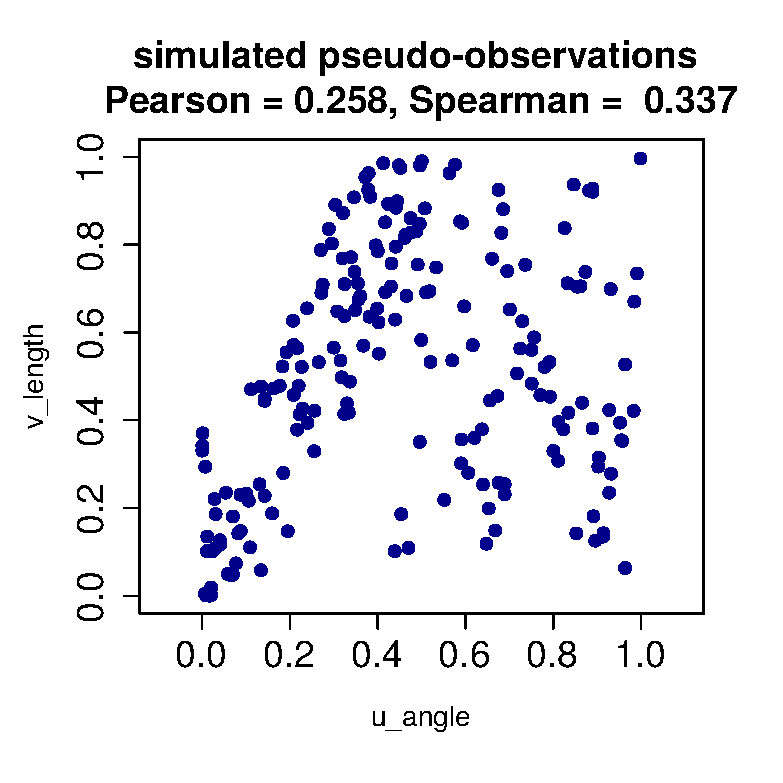
\includegraphics[height=0.4\textwidth,  keepaspectratio = TRUE]{empCopScatter_sim-1}
	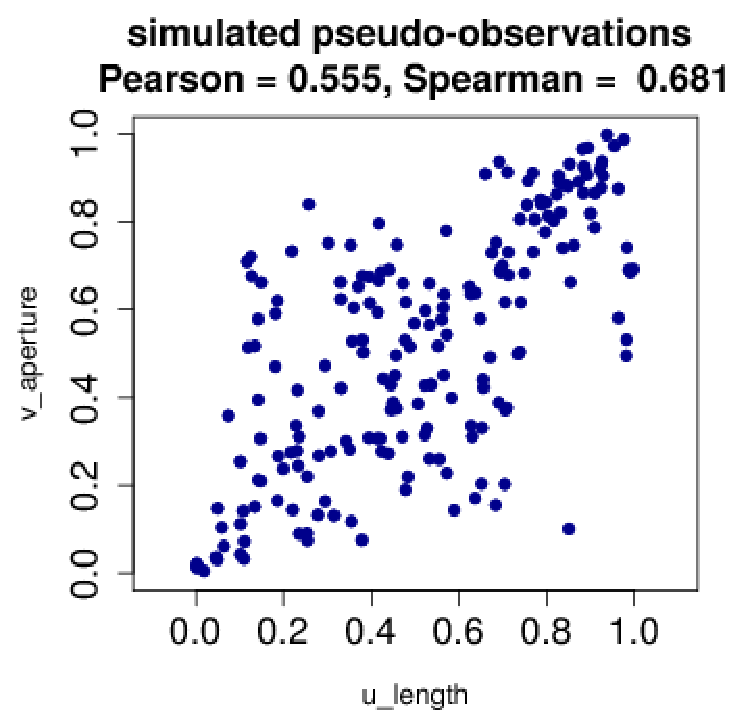
\includegraphics[height=0.4\textwidth,  keepaspectratio = TRUE]{empCopScatter_sim-2}
	\caption{Gr\'afico de pseudo-observaciones simuladas.}
\end{figure}


\section{Resultados y discusi\'on}
\label{sec:results}

Por construcci\'on, el enfoque de Bernstein-Kantorovich para modelar la funci\'on cuantil univariada es no param\'etrico, pero se observaron muy buenos resultados para modelar todas las variables, incluyendo la direcci\'on de las fracturas.
Esto debido a que el problema de la periodicidad se compensa en la modelaci\'on al tener muchos datos en esta frontera.
Las simulaciones con este enfoque univariado reprodujo incluso modas sutiles en los datos.

En la parte bivariada, los diagramas de pseudo-observaciones muestran una correcta correspondencia entre los datos y las simulaciones con las c\'opulas de Bernstein: la mayor\'ia de las fracturas peque\~nas est\'an alineadas en la direcci\'on E-O y las fracturas m\'as grandes en la direcci\'on perpendicular. Los resultados tambi\'en se aprecian en los diagramas de dispersi\'on.

Por el contrario, el diagrama de pseudo-observaciones utilizando la metodolog\'ia est\'andar no imita la dependencia de los datos. A\'un m\'as grave, la mayor\'ia de las fracturas grandes apuntan en la direcci\'on de las fracturas peque\~nas. Incluso hay fracturas grandes en las zonas de probabilidad donde no deber\'ia de haber y tambi\'en fracturas peque\~nas en zonas de casi nula probabilidad de ocurrencia. Por ejemplo, se observan fracturas muy peque\~nas en la direcci\'on N-S, pero en los datos originales no las hay.

Se observ\'o una buena correspondencia tanto en la DFN de los datos como de las simulaciones con la metodolog\'ia propuesta tomando en cuenta la estructura de dependencia. En general, todas las variables involucradas fueron reproducidas, tanto de manera gr\'afica como en sus estad\'igrafos, adem\'as de marginal como de manera conjunta.

Las rosetas y los histogramas para cada una de las simulaciones parecen m\'as suavizados que sus correspondientes de los datos originales. Tal suavizado tambi\'en se reflej\'o de manera cuantitativa en una disminuci\'on de la desviaci\'on est\'andar. Investigando se encontr\'o \citep[p. 251]{phillips_interpolation_2003} que este fen\'omeno se debe a que la convergencia uniforme de los polinomios de Bernstein es muy lenta, o cual se traduce en un suavizado de la curva.

%%  DISCUSSION
%% implications:
Debido a que la relaci\'on orientaci\'on-longitud de fracturas es muy importante en un contexto geol\'ogico y din\'amico, adem\'as de para obtener propiedades de percolaci\'on de un yacimiento naturalmente fracturado dado, esta metodolog\'ia es de mucha utilidad cuando se observan dependencias entre tales variables.

%% limitations:
Este trabajo se ha limitado a desarrollar algoritmos, metodolog\'ia y ejemplos de aplicaci\'on en los casos bivariado y trivariado con c\'opulas de Vine. Sin embargo, se han mostrado algunas f\'ormulas para incluir m\'as de tres variables. En este sentido, \cite{weis_smooth_2012} mostraron c\'omo extender la metodolog\'ia dentro del enfoque de c\'opulas de Vine.

% Otra limitaci\'on fue considerar independencia entre las propiedades de los objetos booleanos y su ubicaci\'on espacial, por ejemplo, la direcci\'on con la intensidad de fracturamiento. N\'otese que esta limitaci\'on est\'a resuelta utilizando los m\'etodos de estimaci\'on espacial multivariada (cokriging por ejemplo) pero est\'a limitado a variables que tienen fuerte correlaci\'on lineal.

Aunque se podr\'ia haber utilizado modelos geoestad\'isticos para la intensidad de fractura se decidi\'o utilizar procesos puntuales con intensidad constante ya que despu\'es de varios intentos, el objeto de estudio de este trabajo (la dependencia entre las propiedades de las fracturas) se analizaba mejor visualmente con un proceso puntual homog\'eneo.

